\chapter{Background}
\label{background}

%2.1-open neuro science
\cite{abrams2021standards}
% 2.1.1 data and tool sharing in neuroscience

% the platfroms that share tools and pipelines , (the infrustructure)  an overview of CONP as well
\MM{WHY I talked about each topic here?...}


In this chapter, in section one we explain what Open Science is, FAIR principles~\cite{FAIR_Principles} which are defined for open science, and how open science can be helpful for researchers and scientists. We will then explain that open science is highly noticeable in neuroscience in section two and will write about some of the existing data and tool sharing platforms which attempt to guarantee FAIR principles~\cite{wilkinson2016fair}. In section three we will explain the recommender systems and the two main strategies.

% , there is no infrastructure which helps researchers in creating relevant analysis from these resources which led us to generate a recommender system for scientific pipelines and datasets.

% we explained the existing open neuroscience platforms, that they apply FAIR principles for the datasets, resources and analysis tools integrated on them. Therefore the user of these platforms has access to the previous analysis stored on the platforms and can run tool or pipeline on a dataset. However, the users are assisted until this phase, and there is no reliable system to help them select the appropriate pipeline and dataset for their analysis. In our project, we investigate the feasibility creating a recommender system to recommend pipelines and datasets based on the records from previous executions. 



\section{Open Science}

Open science is a collection of actions designed to make scientific processes more transparent and results more accessible. Its goal is to build a more replicable and robust science~\cite{spellman_gilbert_corker_2017}. Open science means that all steps in scientific research (including publications, data, physical samples, and software) should be publicly accessible to all levels of an inquiring society, amateur or professional~\cite{woelfle2011open}. In 2016 ‘FAIR Guiding Principles for scientific data management and stewardship’ were published and intended to provide guidelines to improve the Findability, Accessibility, Interoperability, and Reusability of digital assets with the objective of promoting open science. Importantly, these principles apply not only to ‘data’ in the conventional sense, but also to the algorithms, tools, and workflows that led to that data. All scholarly digital research objects (from data to analytical pipelines) benefit from application of these principles, since all components of the research process must be available to ensure transparency, reproducibility, and reusability.

The following explanations about the definitions of FAIR principles is derived from FAIR website~\cite{FAIR_Principles}.  
\subsection*{Findability}
Finding the data is the first step of reusing them so metadata and data should be easy to find for both humans and computers, to achieve that, the metadata should be machine-readable for automatic discovery of datasets and services.
Findability includes four principles:
\subsubsection*{F1. (Meta)data are assigned a globally unique and persistent identifier}
It is essential for data or metadata to be assigned a globally unique and persistent identifier to remove ambiguity, make findability more feasible and help others for the citation when they reuse the data. Some data repositories will automatically generate such identifiers for the deposited datasets

\subsubsection*{F2. Data are described with rich metadata}
Rich metadata means that the description of the data should include information about the context, quality and condition, or characteristics of the data therefore users will be able to find data based on the information provided by their metadata, even without the data’s identifier.

\subsubsection*{F3. Metadata clearly and explicitly include the identifier of the data they describe}
This principle is critically important since usually the metadata and the data itseld are in seperate files, therefore the association between them should be made explicit by mentioning a dataset’s globally unique and persistent identifier in the metadata. 
\subsubsection*{F4. (Meta)data are registered or indexed in a searchable resource}
To ensure 'findability' the data and resources should be discoverable using indexing which will be achieved by F1-F3.

\subsection*{Accessibility}
After finding the data, the user needs to know how to access or get the data, to make it happen there are two required principles:

\subsubsection*{A1. (Meta)data are retrievable by their identifier using a standardised communications protocol}
To make the (meta)data retrievable, the protocol is required to guarantee the following principles: 

\quad A1.1.The protocol should be open, free, and universally implementable to facilitate data retrieval so that anyone with a computer and an internet connection can access at least the metadata.

\quad A1.2. The protocol should allow for an authentication and authorisation procedure, where necessary. Meaning that, accessibility does not necessary mean 'open' or 'free', and it is required for the data repositories to provide the conditions or instructions under which the data will be accessible. Creating an account in repositories for the data user for instance.

\subsubsection*{A2. Metadata are accessible, even when the data are no longer available}  Accessibility of metadata is related to the registration and indexing issues described in F4. 


\subsection*{Interoperability}
The data usually need to be integrated with other data or inter-operate with applications or workflows for analysis, storage, and processing, to make it happen it is required that:


\subsubsection*{I1. (Meta)data use a formal, accessible, shared, and broadly applicable language for knowledge representation}

"Interoperability typically means that each computer system at least has knowledge of the other system’s data exchange formats"~\cite{FAIR_Principles}. To make this happen it is required to use commonly used controlled vocabularies, anthologies, and a good data model to describe and structure (meta)data.
 
\subsubsection*{I2. (Meta)data use vocabularies that follow FAIR principles}
% The controlled vocabulary used to describe datasets needs to be documented and resolvable using globally unique and persistent identifiers. This documentation needs to be easily findable and accessible by anyone who uses the dataset.

\subsubsection*{I3. (Meta)data include qualified references to other (meta)data}
It should be specified in the metadata if one dataset builds on another dataset, or if additional datasets are required to complete the data, or if complementary information is stored in a different dataset. In particular, the scientific links between the datasets need to be described.

\subsection*{Reusability}
To achieve the final principle in FAIR it is required that:

\subsubsection*{R1. (Meta)data are richly described with a plurality of accurate and relevant attributes}
It would be much easier to find and reuse data if metadata includes many labels, R1 is related to F2, however, R1 means if the user or machine is able to decide if the data is actually 'useful' in a particular context. Therefore, metadata should richly describes the context under which the data was generated. 

\quad R1.1. (Meta)data are released with a clear and accessible data usage license,

% Under ‘I’, we covered elements of technical interoperability. R1.1 is about legal interoperability. What usage rights do you attach to your data? This should be described clearly. Ambiguity could severely limit the reuse of your data by organisations that struggle to comply with licensing restrictions. Clarity of licensing status will become more important with automated searches involving more licensing considerations. The conditions under which the data can be used should be clear to machines and humans.


\quad R1.2. (Meta)data are associated with detailed provenance

% For others to reuse your data, they should know where the data came from (i.e., clear story of origin/history, see R1), who to cite and/or how you wish to be acknowledged. Include a description of the workflow that led to your data: Who generated or collected it? How has it been processed? Has it been published before? Does it contain data from someone else that you may have transformed or completed? Ideally, this workflow is described in a machine-readable format.

\quad R1.3. (Meta)data meet domain-relevant community standards

% It is easier to reuse data sets if they are similar: same type of data, data organised in a standardised way, well-established and sustainable file formats, documentation (metadata) following a common template and using common vocabulary. If community standards or best practices for data archiving and sharing exist, they should be followed. For instance, many communities have minimal information standards (e.g., MIAME, MIAPE). FAIR data should at least meet those standards.  Other community standards may be less formal, but nevertheless, publishing (meta)data in a manner that increases its use(ability) for the community is the primary objective of FAIRness. In some situations, a submitter may have valid and specified reasons to divert from the standard good practice for the type of data to be submitted. This should be addressed in the metadata. Note that quality issues are not addressed by the FAIR principles. The data’s reliability lies in the eye of the beholder and depends on the intended application.



\section{Open neuroscience}
In the world of neuroscience a lot of attempts have been
 made to simplify reproducible research, specifically in neuroimaging, and functional Magnetic Resonance Imaging (fMRI)\cite{Schottner_2020}. Also it is important for such platforms to satisfy FAIR principles. Among the existing platfroms for open neuroscience, we introduce OpenNuero, NeuroImaging Tools \& Resources Collaboratory (NITRIC) and Canadian Open Neuroscience Platform (CONP).


\subsection{OpenNeuro}
\href{https://openneuro.org}{OpenNeuro}, formerly known as OpenfMRI\cite{poldrack2017openfmri}, is a free online platform for storing, sharing and analysing of neuroimaging data~\cite{gorgolewski2017openneuro}. Researchers can upload their own data to share it with others and download others shared data, also they can run analysis pipelines on the data. 

\subsubsection{Uploading and sharing the data}
 OpenNeuro only accepts BIDS~\cite{gorgolewski2016brain} compatible datasets,(MRI, MEG, EEG, iEEG, ECoG, ASL, and PET data), and all datasets will by validated to be BIDS compatible before being uploaded. In OpenNeuro, when uploading data, users can specify if their data will be accessible publicly or not, however, the user agrees that the uploaded data on will be publicly accessible after 18 months. After uploading the data on OpenNeuro, the users are able to change the dataset, change metadata, apply versioning on the dataset or make copies of the dataset to guarantee the reputability of analysis. 
 
 The users can share their uploaded data with other colleagues or researchers and specify the level of access ranging from viewing to administration 

\subsubsection{Running analysis on the data }
The most exiting feature of OpenNeuro is that the users are able to run different analysis on the data and share the results of that. The user can select one of the containerized analysis pipelines among all available BIDS Apps to apply on the dataset. The only applicable tools are BIDS Apps~\cite{gorgolewski2017bids} since, as mentioned above, OpenNeuro accept only BIDS compatible dataset. After selecting a BIDS App, the user can set parameters and specify if the analysis should run on the whole dataset or on specific subject or sessions. Then the user can download all the generated results, use them for higher level costume analysis and the will have access to all logs for the executed analysis and will be able to debug the process if it has failed.


\subsection{NeuroImaging Tools and Resources Collaboratory (NITRIC)} 
The Neuroimaging Informatics Tools and Resources Collaboratory
(\href{www.nitrc.org}{NITRIC}) provides a triad of services include a Resources Registry (NITRIC-R), Image Repository (NITRIC-IR) and a cloud Computational Environment (NITRIC-CE) to meet the needs of the neuroimaging researchers\cite{kennedy2016nitrc,howToCiteNITRIC_website}\MM{how to cite nitric website as they mentioned?}.



% NITRC provides image-sharing functionality through both the NITRC Resource
% Registry (NITRC-R), where bulk data files can be released through the file release system (FRS), and the NITRC
% Image Repository (NITRC-IR), a XNAT-based image data management system. Currently hosting 14 projects,
% 6845 subjects, and 8285 MRI imaging sessions, NITRC-IR provides a large array of structural, diffusion and resting
% state MRI data.
\subsubsection{NITRIC-R}

Resources, in this case, are broadly defined to include software, hardware, data,
websites, community organizations, etc. NITRC-R gives researchers greater and more efficient access to the tools and resources they need, better categorizing and organizing existing tools and resources, facilitating interactions between researchers and developers, and promoting better use through enhanced documentation and tutorials, forums, and updates. 

Each NITRC project has a homepage that describes the resources, provides
a standard set of resource characteristics (i.e. keywords, license,
dependencies, etc.), and provides a standard set of links for the resources
(i.e. download, documentation, support, etc.). Each resource page is
maintained by the resource administrator, who is responsible for
keeping it up to date. For every
project, resource administrators are also free to enable/disable any
functionality and redirect any content to other sources, as pertinent to
the resource developers' needs. Visitors to the NITRC site can search
for resources based on keywords, free text and specific capabilities in
order to find relevant resources. Currently, there are more that 1200 registered tools and 43000 registered users in NITRIC-R. 

\subsubsection{NITRIC-IR}

NITRC Image Repository offers a cloud-based federated neuroimaging data storage system for resource sharing of neuroimaging data in DlCOM and NIfTI formats. Currently it includes thousands of subjects and imaging sessions searchable across over a dozen projects to promote re-use and integration of valuable NIH-funded data.

The NITRC-IR is built on XNAT~\cite{marcus2007extensible} and provides sharing infrastructure for images and related data that can be closely integrated with the NITRC-R resources in order to better, support, promote, and manage data sharing functions for NITRC-hosted projects.
NITRC-R projects can be associated with NITRC-IR (XNAT) ‘projects’ and these can be interlinked. 
% From the search results you may select and download images. NITRC's Image Repository leverages XNAT software: Extensible Neuroimaging Archive Toolkit. 


\subsubsection{NITRIC-CE}

The NITRC Computational Environment is a freely downloadable, virtual computing cloud-based platform built upon a NeuroDebian operating system. NITRC-CE preinstalls popular neuroimaging tools such as AFNI, ANTS, FreeSurfer, FSL, C-PAC, and MRIcron (for the complete list of tools click \href{https://www.nitrc.org/plugins/mwiki/index.php/nitrc:User_Guide_-_NITRC-CE_Installed_Packages}{here}) into a standardized computational environment to help users analyze their data quickly and easily. This environment can be deployed in the cloud (using Amazon Web Services Elastic Compute Cloud (EC2) or the Microsoft Azure Cloud Computing Platform), or as a virtual machine for local use. To run analysis, NITRIC-CE can access data through NITRIC-IR, NITRIC-R, secure file transfer from outside sources, and file system mounting of AWS S3 resources.


% \subsubsection{Access and data sharing in NITRIC}
% Each NITRC project manages its own access policy. Data, in either
% NITRC-R or NITRC-IR can be completely open, not requiring any
% authentication; open to NITRC users; or open only to NITRC users who
% are registered with a specific project. 

% Data sharing within the NITRC-R is supported by the file release system (FRS) which provides support for release of packages, releases and files. Data sharing within the NITRC-IR is build around projects, subjects, sessions and assessors, and data access for the NITRC-CE is facilitated through access to NITRC-IR and NITRC-R.








\section{Recommender Systems}

Recommender System or recommendation system is included in the information filtering systems which aim at providing suggestions for items to a user by predicting the 'rating' or 'preference' a user would give to an item\cite{isinkaye2015recommendation,ricci2011introduction}. These suggestions might come out of various decision-making processes, whether or not to buy an item, listen to a piece of music or read an article. Also, 'item' is a general purpose term referring to what the system will recommend to its users, for instance it can be software tool, news or magazine, and products to purchase. The definitions provided in the rest of this section are mostly summary of chapter 9 of 'Mining of Massive Datasets'~\cite{rajaraman2011mining}.

Currently, the recommender systems can be seen in anywhere that there exists a possible user who needs to decide to choose an 'item'. From the most popular recommendation systems we can point to product recommendations, movie recommendations and news and article recommendations. In product recommendations, online retailers such as Amazon are increasingly attempting to attract and keep their users with suggesting more relevant product that they might like to buy. This will lead to a win-win outcome, finding relevant products for the users and increasing the revenue for the business owners. Another application of recommender systems is movie recommendations such as Netflix, which recommends its users the movies or TV shows that they might like based on many factors such as previous watched movies, the ratings (currently 'like' or 'dislike') given or the similar users' choices. There are so many other factors that helps Netflix to provide good suggestions for its users. Another application of recommender systems can be in news and articles, "news services have attempted to identify articles of interest to readers, based on the articles that they have read in the past. The similarity might be based on the similarity of important words in the
documents, or on the articles that are read by people with similar reading
tastes. The same principles apply to recommending blogs from among
the millions of blogs available, videos on YouTube, or other sites where content is provided regularly"~\cite{rajaraman2011mining}.





There are several technologies in recommender systems to find the best 'item' for a 'user' that we can classify them in two broad groups, Content-based and Collaborative filtering \cite{rajaraman2011mining}. In a content-based recommender system focuses on item/user profile which describes a set of features and properties of that item/user. Then recommends an item to a user if it is similar to the previous choices of the user. However, a Collaborative filtering recommender system focuses on the relationship between users and items; an items will be recommended to a user if it is preferred by similar users. 

Before going through detailed explanations of Content-based and Collaborative Filtering recommendation approaches, we need to define the Utility Matrix and its role in recommendation approaches. 
\subsection{Utility Matrix}
In the recommender systems 'user' and 'item' are the terms used to represent the two main classes of entities.  The Utility Matrix is indexed with users' ids on one axis and items' on the other and includes values assigned to each pair of user-item which represents the user's preference for the item. In this case, values might represent the item's rating given by the user, 1-5 stars for example. Usually, the utility matrix is sparse, meaning that the rating value for most of the user-item pairs are 'unknown', which implies that there have not been explicit information about the user's preference for that item. 
%, or the number of time a user has selected the item ( >= 0), for instance the number of downloads, views or buying an item.

Figure~\ref{fig:utilityMatrix} is an example in which the utility matrix represents the ratings (1-5) for movies (HP1, HP2, and HP3 for Harry Potter I, II, and III, TW for Twilight, and SW1,
SW2, and SW3 for Star Wars episodes 1, 2, and 3) given by the users (A,B,C,D). The blank units represents unknowns, in which the user has not rated the movie. In practice, the utility matrices are mostly sparser than this matrix, since there is a small fraction of real users who give explicit feedback on items. The goal of the recommender system is to predict the value for the blanks in the utility matrix.

% We should also be aware of a slightly different goal that makes sense in
% many applications. It is not necessary to predict every blank entry in a utility
% matrix. Rather, it is only necessary to discover some entries in each row that
% are likely to be high. In most applications, the recommendation system does
% not offer users a ranking of all items, but rather suggests a few that the user
% should value highly. It may not even be necessary to find those items with
% the highest expected ratings, but only to find a large subset of those with the
% highest ratings.

\begin{figure*}[ht]
  \centering
  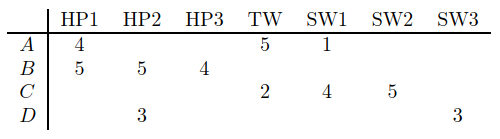
\includegraphics[width=\textwidth]{figures/utilityMatrix.png}
  \caption{A utility matrix representing ratings of movies on a 1–5 scale. The figure is derived from chapter 9 of MMDS book~\cite{rajaraman2011mining}}
  \label{fig:utilityMatrix}
\end{figure*} 


The utility matrix is the most important requirement to generate a recommendation system. However, it is usually difficult to acquire data from users for the utility matrix. There are two general approaches to gather data from users, first by asking them to rate the items. For instance, asking them to rate after watching a movie or buying a product. However, this this approach is not effective, "since generally
users are unwilling to provide responses, and the information from those
who do may be biased by the very fact that it comes from people willing
to provide ratings"~\cite{rajaraman2011mining}. Another approach would be data acquisition from users interactions and behaviour. For instance, if a user
buys a product, watches a movie, or reads an article, it represents that they 'liked' that item. For this sort of rating the only value is 1 (for getting user's response) and the unknown pairs would be 0; in this case 0 is not lower that 1, it is no rating at all.

\subsection{Content based}
Content-based recommender systems focus on the item's properties described in its profile and then recommends a user the similar items to the ones they 'liked' before. Similarity between items will be gained by measuring the similarity between their profiles. Users also can have their profiles describing their properties.

In this section we will explain item and user profiles, how to gather the information from different types of items and how exactly the content-based recommendation system works. 

\subsubsection{Item profile}




\subsection{Collaborative filtering}
Collaborative filtering approach for recommender systems, focuses on user-item interactions. There are three main categories of Collaborative Filtering, Memory-based, Model-based and Hybrid CF. Neighbor-based CF (kNN) and Latent semantic CF are well known techniques in Memory-based and Model-based categories respectively  [X Su 2009]. In Neighbor-based CF the goal is to identify like-minded users based on similarity of their item ratings or purchasing history, moreover, finding items that are rated similarly would be another goal in this technique [Y Koren 2007]. In Latent factor (Latent semantic CF or Factorization-based) model, the observation (rating) matrix is modeled as a product of a user factor matrix and an item factor matrix [S Girase, 2015], and the goal is to estimate the missing user-item pair value (user feedback) by calculating latent features that accurately describe the interaction between users and items [Y Koren 2011]. A popular and accurate method in latent factor model is Singular Value Decomposition (SVD), where each user and item is represented by a factor vector, and the prediction is done by computing the inner product of these vectors  [Y Koren 2008]. 
All collaborative filtering techniques work by user actions or feedback, user feedback data is divided in two main categories, explicit feedback and implicit feedback. Explicit feedback points to capturing user preferences in a explicit and direct way, such as rating movies, which is a difficult to get approach. However, implicit feedback, refers to all recorded behaviour of user which illustrates their preference, this type of feedback can be easily available  [Nathan N. Liu 2010]. 



